
% Copyright (c) 2015 - 2020 Mario Mlačak, mmlacak@gmail.com
% Public Domain work, under CC0 1.0 Universal Public Domain Dedication. See LICENSING, COPYING files for details.

% Miranda's veil chapter ==============================================
\chapter*{Miranda's veil}
\addcontentsline{toc}{chapter}{Miranda's veil}
\label{ch:Miranda's veil}

\begin{flushright}
\parbox{0.8\textwidth}{
\emph{Under all that we think, lives all we believe, like the ultimate veil of our spirits. \newline
\hspace*{\fill}{\textperiodcentered \textperiodcentered \textperiodcentered \hspace*{0.2em} Antonio Machado} } }
\end{flushright}

\noindent
Miranda's veil is chess variant which is played on 16 x 16 board, with
white and dark violet fields and light magenta and indigo pieces.
A new piece is introduced, Wave.

\clearpage % ..........................................................
% Wave ****************************************************************

\section*{Wave}
\addcontentsline{toc}{section}{Wave}
\label{sec:Miranda's veil/Wave}

\vspace*{-1.4\baselineskip}
\noindent
\begin{wrapfigure}[12]{l}{0.4\textwidth}
\centering
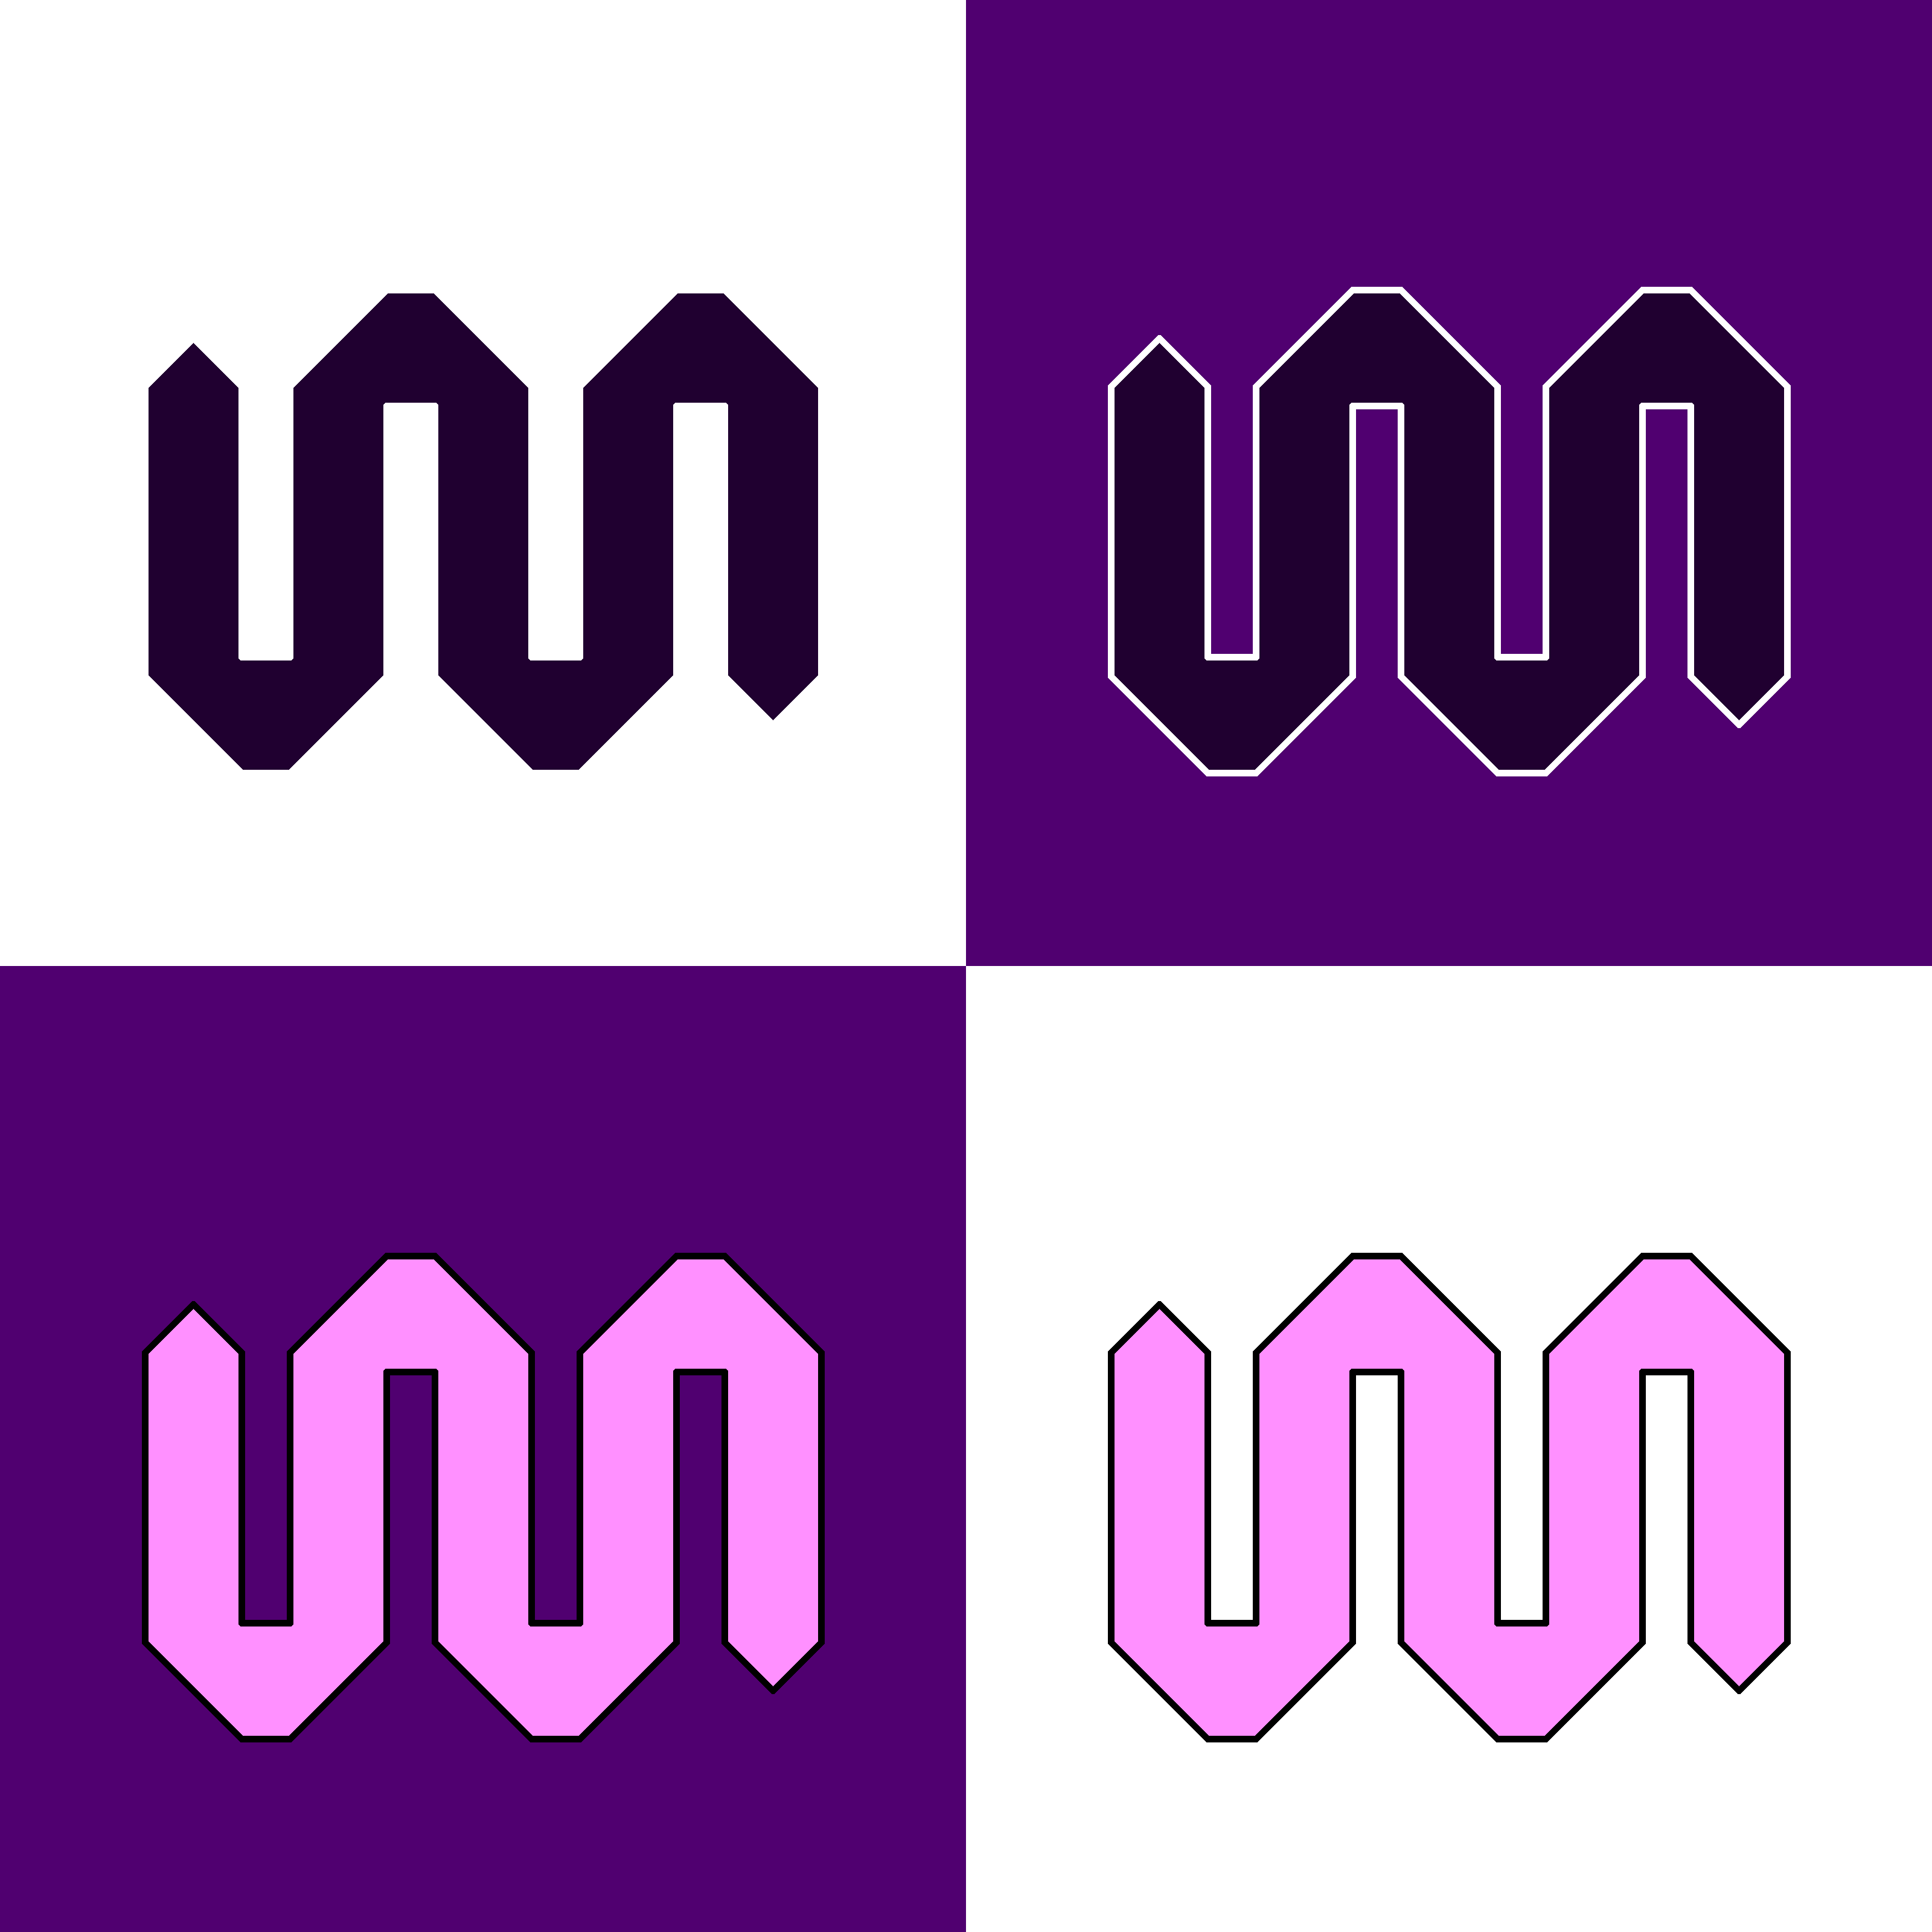
\includegraphics[width=0.4\textwidth, keepaspectratio=true]{pieces/10_wave.png}
\caption{Wave}
\label{fig:10_wave}
\end{wrapfigure}
Wave is passive piece, it has to be activated before it can move. Activation is done
with own piece capturing field at which Wave is located, before Wave can move.
Movement of Wave mimics that of activating piece, and is not limited to a single
step.

Wave does not use received momentum for moving, and so Wave can be activated even
with no momentum. Wave can activate any own piece, except King, if it has momentum.
Wave can also activate other Wave, own or opponent's, even if it has no momentum.
Wave transfers all of received momentum to a piece it activates.

Wave is transparent; all other pieces can move past (pass over) Wave, as if it
isn't present on a chessboard. Other pieces are transparent to Wave; Wave can move
past (pass over) any piece, as if it isn't there. Transparency of Wave makes
activation of Wave optional.

Wave cannot capture any piece; and so cannot neither check nor checkmate opponent's
King.

\clearpage % ..........................................................
% Activation ----------------------------------------------------------

\subsection*{Activation}
\addcontentsline{toc}{subsection}{Activation}
\label{sec:Miranda's veil/Wave/Activation}

\vspace*{-1.4\baselineskip}
\noindent
\begin{figure}[!h]
\includegraphics[width=1.0\textwidth, keepaspectratio=true]{examples/10_mv/scn_mv_01_wave_activation_init.png}
\vspace*{-1.3\baselineskip}
\caption{Activating Wave}
\label{fig:scn_mv_01_wave_activation_init}
\end{figure}

\vspace*{-0.3\baselineskip}
A piece can activate own Wave by simply capturing a field at which that Wave stands.
Activation is optional, a piece could just as well move past Wave. Activated Wave
receives any momentum activating piece had.

Here, Pegasus has opportunity to activate Wave, with 5 momentum.

\clearpage % ..........................................................

\vspace*{-2.1\baselineskip}
\noindent
\begin{figure}[!h]
\includegraphics[width=1.0\textwidth, keepaspectratio=true]{examples/10_mv/scn_mv_02_wave_activated.png}
\caption{Wave activated}
\label{fig:scn_mv_02_wave_activated}
\end{figure}

Activated Wave inherits way of moving from the activating piece. Activated Wave
does not spend received momentum for moving, and so Wave can be activated even if
activating piece has no momentum.

Here, Wave activated by Pegasus (now "in the air") moves like one, i.e. along one
chosen semi-diagonal.

\clearpage % ..........................................................
% Activating pieces ...................................................

\subsubsection*{Activating pieces}
\addcontentsline{toc}{subsubsection}{Activating pieces}
\label{sec:Miranda's veil/Wave/Activation/Activating pieces}

\vspace*{-1.5\baselineskip}
\noindent
\begin{figure}[!h]
\includegraphics[width=1.0\textwidth, keepaspectratio=true]{examples/10_mv/scn_mv_03_pawn_pass_through.png}
\vspace*{-1.4\baselineskip}
\caption{Passing opponent's Pawn}
\label{fig:scn_mv_03_pawn_pass_through}
\end{figure}

\vspace*{-0.5\baselineskip}
Wave in its movement is not obstructed by any piece on chessboard, it can move
past (pass over) any piece, as if it's not there. In short, other pieces are
all transparent to Wave, and all activations are optional.

Here, Wave cannot activate opponent's Pawn on its step-field, but it's not
hindered by that Pawn, and can reach fields behind it, which would be out of
reach for Pegasus.

\clearpage % ..........................................................

\vspace*{-2.1\baselineskip}
\noindent
\begin{figure}[!h]
\includegraphics[width=1.0\textwidth, keepaspectratio=true]{examples/10_mv/scn_mv_04_wave_activating_rook.png}
\vspace*{-1.3\baselineskip}
\caption{Activating Rook}
\label{fig:scn_mv_04_wave_activating_rook}
\end{figure}

\vspace*{-0.3\baselineskip}
Wave can activate any own piece, except King, if it has momentum. Wave can also
activate any other Wave, own or opponent's, even if it doesn't have any momentum.
Wave does not spend received momentum while moving, and would transfer it entirely
to any piece it activates.

Here, Wave can activate own Rook, even though it's positioned behind opponent's
Pawn, and transfer to it all of 5 received momentum.

\clearpage % ..........................................................

\vspace*{-2.1\baselineskip}
\noindent
\begin{figure}[!h]
\includegraphics[width=1.0\textwidth, keepaspectratio=true]{examples/10_mv/scn_mv_05_rook_activated.png}
\vspace*{-1.3\baselineskip}
\caption{Rook activated}
\label{fig:scn_mv_05_rook_activated}
\end{figure}

\vspace*{-0.3\baselineskip}
Material is any piece, except Wave. Activated material moves the same as it would
in a normal move, i.e. if not activated. The only difference is that activated
material is limited by received momentum, i.e. can't move for more fields than
momentum it received.

Here, activated Rook (now "in the air") can choose one of horizontals or verticals
as its new direction. Rook can reach at most 5 fields, because that's the momentum
it received.

\clearpage % ..........................................................

\vspace*{-2.1\baselineskip}
\noindent
\begin{figure}[!h]
\includegraphics[width=1.0\textwidth, keepaspectratio=true]{examples/10_mv/scn_mv_06_rook_captures.png}
% \vspace*{-1.3\baselineskip}
\caption{Rook captures}
\label{fig:scn_mv_06_rook_captures}
\end{figure}

Activated material piece can also capture opponent's piece, if it's within reach,
and not obstructed by other pieces.

Here, activated Rook can capture dark Knight; it can't capture dark Bishop since
own light Pawn is in the way. Light Rook can't capture dark Pegasus since it's out
of reach.

% ................................................... Activating pieces
\clearpage % ..........................................................
% Wave is transparent .................................................

\subsubsection*{Wave is transparent}
\addcontentsline{toc}{subsubsection}{Wave is transparent}
\label{sec:Miranda's veil/Wave/Cascading Waves/Wave is transparent}

\vspace*{-1.4\baselineskip}
\noindent
\begin{figure}[!h]
\includegraphics[width=1.0\textwidth, keepaspectratio=true]{examples/10_mv/scn_mv_07_wave_is_transparent.png}
\vspace*{-1.3\baselineskip}
\caption{Wave is transparent}
\label{fig:scn_mv_07_wave_is_transparent}
\end{figure}

\vspace*{-0.4\baselineskip}
Just as other pieces are transparent to Wave, so is Wave transparent for all the
other pieces. Any interaction with a Wave is optional; a piece could activate own
Wave, it could capture opponent's Wave, or it could move past all Waves in its path,
and e.g. capture opponent's piece behind a Wave.

\noindent
Here, light Queen could interact with any Wave in her path, or capture dark Pegasus;
dark Pawn is shielded by own Pegasus.

\clearpage % ..........................................................

\vspace*{-2.1\baselineskip}
\noindent
\begin{figure}[!h]
\includegraphics[width=1.0\textwidth, keepaspectratio=true]{examples/10_mv/scn_mv_08_wave_cant_be_pinned.png}
\vspace*{-1.3\baselineskip}
\caption{Wave is not pinned}
\label{fig:scn_mv_08_wave_cant_be_pinned}
\end{figure}

\vspace*{-0.5\baselineskip}
Since it's transparent Wave cannot be pinned, i.e. a piece can ignore (pass over)
Wave placed on its capture-field, and still check opponent's King.

Here, dark Pegasus checks light King, even though light Wave is on dark Pegasus'
capture-field. Any other piece positioned instead of light Wave would be
\href{https://en.wikipedia.org/wiki/Pin_(chess)#Absolute_pin}{hard-pinned},
and light King wouldn't be in check.

% ................................................. Wave is transparent
\clearpage % ..........................................................

\subsubsection*{Wave and castling}
\addcontentsline{toc}{subsubsection}{Wave and castling}
\label{sec:Miranda's veil/Wave/Cascading Waves/Wave and castling}

\vspace*{-0.4\baselineskip}
Wave is transparent, so it doesn't block castling if positioned between castling
pieces and their destination fields. Wave cannot be activated by castling piece,
so it blocks any castling which uses its field as a destination.

\vspace*{-0.4\baselineskip}
\noindent
\begin{figure}[!h]
\includegraphics[width=1.0\textwidth, keepaspectratio=true]{examples/10_mv/scn_mv_09_wave_no_block_castling_king.png}
\vspace*{-1.4\baselineskip}
\caption{Castling King}
\label{fig:scn_mv_09_wave_no_block_castling_king}
\end{figure}

\vspace*{-1.4\baselineskip}
\noindent
\begin{figure}[!h]
\includegraphics[width=1.0\textwidth, keepaspectratio=true]{examples/10_mv/scn_mv_10_wave_no_block_castling_rook.png}
\vspace*{-1.4\baselineskip}
\caption{Castling Rook}
\label{fig:scn_mv_10_wave_no_block_castling_rook}
\end{figure}

\vspace*{-0.4\baselineskip}
In previous example King initiated castling by moving onto a field past Wave, Rook
can now finish castling onto empty field between the two, so the whole castling move
is legal.

\vspace*{-0.4\baselineskip}
\noindent
\begin{figure}[!h]
\includegraphics[width=1.0\textwidth, keepaspectratio=true]{examples/10_mv/scn_mv_11_wave_block_castling_rook.png}
\vspace*{-1.4\baselineskip}
\caption{Castling Rook blocked}
\label{fig:scn_mv_11_wave_block_castling_rook}
\end{figure}

\vspace*{-0.4\baselineskip}
If in previous example King initiated castling by moving onto a field just past Wave,
Rook cannot castle onto field occupied by Wave, so the whole castling move is illegal.

\clearpage % ..........................................................

\subsubsection*{Single-step pieces and transparency}
\addcontentsline{toc}{subsubsection}{Single-step pieces and transparency}
\label{sec:Miranda's veil/Wave/Cascading Waves/Single-step pieces and transparency}

\vspace*{-0.7\baselineskip}
\noindent
\begin{wrapfigure}[13]{l}{0.4\textwidth}
\centering
\includegraphics[width=0.39375\textwidth, keepaspectratio=true]{examples/10_mv/scn_mv_12_pawn_blocked_by_opponents_wave.png}
\vspace*{-1.4\baselineskip}
\caption{Pawns blocked by Waves}
\label{fig:scn_mv_12_pawn_blocked_by_opponents_wave}
\end{wrapfigure}
Image on the left and the next one both have two examples presented in parallel,
each started by a labeled Pawn. \newline
\indent
To use transparency, a piece has to be able to reach a Wave, and then make another
step away from it, in the same ply. So, single-step piece (i.e. a Pawn, Knight, King,
or Unicorn) has to activate own, or capture opponent's Wave; otherwise it's blocked
by a Wave, regardless if own, or opponent's.

\vspace*{1.1\baselineskip}
\noindent
\begin{wrapfigure}[16]{l}{0.4\textwidth}
\centering
\includegraphics[width=0.39375\textwidth, keepaspectratio=true]{examples/10_mv/scn_mv_13_pawn_not_blocked_by_opponents_wave.png}
\vspace*{-1.4\baselineskip}
\caption{Pawns not blocked by Waves}
\label{fig:scn_mv_13_pawn_not_blocked_by_opponents_wave}
\end{wrapfigure}
In previous example light Pawn B is blocked from moving straight forward by dark
Wave on its step-field; other Waves can be either activated, or captured. No Wave
can be passed over, since both Pawns can make only one step in a ply. \newline
\indent
Here, both Pawns can rush, thus making more than one step in a single ply. Opponent's,
dark Wave is blocking light Pawn B from settling onto step-field it occupies. Even so,
both Waves are transparent to light Pawns; each Pawn can now pass over corresponding
Wave, and reach step-fields behind it.

\clearpage % ..........................................................

\subsubsection*{Piece blocked}
\addcontentsline{toc}{subsubsection}{Piece blocked}
\label{sec:Miranda's veil/Wave/Activation/Piece blocked}

\vspace*{-1.4\baselineskip}
\noindent
\begin{figure}[h]
\includegraphics[width=1.0\textwidth, keepaspectratio=true]{examples/10_mv/scn_mv_14_wave_no_activating_blocked_piece.png}
\caption{Piece blocked}
\label{fig:scn_mv_14_wave_no_activating_blocked_piece}
\end{figure}

Wave cannot activate blocked pieces, even if it has momentum. Here, Pawn is blocked
from moving forward by own Bishop, and there are no opponent's pieces on its
diagonal capture-fields. So, Wave cannot activate Pawn, even though it has one
momentum received from Knight.

% ---------------------------------------------------------- Activation
\clearpage % ..........................................................
% Movement ------------------------------------------------------------

\subsection*{Movement}
\addcontentsline{toc}{subsection}{Movement}
\label{sec:Miranda's veil/Wave/Movement}

\vspace*{-1.4\baselineskip}
\noindent
\begin{figure}[h]
\includegraphics[width=1.0\textwidth, keepaspectratio=true]{examples/10_mv/scn_mv_15_bishop_activating_wave.png}
\caption{Bishop activating Wave}
\label{fig:scn_mv_15_bishop_activating_wave}
\end{figure}

Generally, activated Wave inherits way of movement from activating piece. Wave activated
by pieces which move for one field (such as Pawn, Knight, King, and Unicorn) can move
over multiple fields. Again, activating Wave is optional, activating piece could continue
its movement past Wave. Activated Wave is not limited by received momentum, and can move
past any piece as if it's not there.

\clearpage % ..........................................................

\vspace*{-2.1\baselineskip}
\noindent
\begin{figure}[!h]
\includegraphics[width=1.0\textwidth, keepaspectratio=true]{examples/10_mv/scn_mv_16_wave_activated_by_bishop.png}
% \vspace*{-1.3\baselineskip}
\caption{Wave activated by Bishop}
\label{fig:scn_mv_16_wave_activated_by_bishop}
\end{figure}

Here, Wave (now "in the air") activated by Bishop moves like one, i.e. along one chosen
diagonal. Activated light Wave cannot activate dark Knight, but can activate own Pawn.
Wave is not obstructed by neither Pawn nor Knight, and can move past them. Wave is not
limited by 4 received momentum, and can reach edge of chessboard.

\clearpage % ..........................................................
% Activated by Knight .................................................

\subsubsection*{Activated by Knight}
\addcontentsline{toc}{subsubsection}{Activated by Knight}
\label{sec:Miranda's veil/Wave/Movement/Activated by Knight}

\vspace*{-1.4\baselineskip}
\noindent
\begin{figure}[h]
\includegraphics[width=1.0\textwidth, keepaspectratio=true]{examples/10_mv/scn_mv_17_knight_activating_wave.png}
\caption{Knight activating Wave}
\label{fig:scn_mv_17_knight_activating_wave}
\end{figure}

Wave can make multiple steps in a ply, even if activated by a piece which can make only
one step. Activated Wave can take one chosen direction, which cannot be changed later.

Here, Knight is about to activate Wave, and transfer to it one momentum.

\clearpage % ..........................................................

\vspace*{-2.1\baselineskip}
\noindent
\begin{figure}[!h]
\includegraphics[width=1.0\textwidth, keepaspectratio=true]{examples/10_mv/scn_mv_18_wave_activated_by_knight.png}
\caption{Wave activated by Knight}
\label{fig:scn_mv_18_wave_activated_by_knight}
\end{figure}

Here, Wave (now "in the air") activated by light Knight can choose one semi-diagonal
(corresponding to steps Knight can make), and then move over multiple step-fields, up
to the edge of chessboard. So, Wave activated by Knight moves like a Pegasus.

% ................................................. Activated by Knight
\clearpage % ..........................................................
% Activated by King ...................................................

\subsubsection*{Activated by King}
\addcontentsline{toc}{subsubsection}{Activated by King}
\label{sec:Miranda's veil/Wave/Movement/Activated by King}

\vspace*{-1.4\baselineskip}
\noindent
\begin{figure}[h]
\includegraphics[width=1.0\textwidth, keepaspectratio=true]{examples/10_mv/scn_mv_19_king_activating_wave.png}
\caption{King activating Wave}
\label{fig:scn_mv_19_king_activating_wave}
\end{figure}

Similarly, Wave activated by King can choose one direction along diagonals, horizontal
or vertical lines (corresponding to steps King can make).

\clearpage % ..........................................................

\vspace*{-2.1\baselineskip}
\noindent
\begin{figure}[!h]
\includegraphics[width=1.0\textwidth, keepaspectratio=true]{examples/10_mv/scn_mv_20_wave_activated_by_king.png}
% \vspace*{-1.3\baselineskip}
\caption{Wave activated by King}
\label{fig:scn_mv_20_wave_activated_by_king}
\end{figure}

Then, Wave (now "in the air") activated by King can move over multiple step-fields,
up to the edge of chessboard. Direction taken by activated Wave cannot be changed
for duration of a ply. So, Wave activated by King moves like a Queen.

% ................................................... Activated by King
\clearpage % ..........................................................
% Activated by Pawn ...................................................

\subsubsection*{Activated by Pawn}
\addcontentsline{toc}{subsubsection}{Activated by Pawn}
\label{sec:Miranda's veil/Wave/Movement/Activated by Pawn}

\vspace*{-1.5\baselineskip}
\noindent
\begin{figure}[!h]
\includegraphics[width=1.0\textwidth, keepaspectratio=true]{examples/10_mv/scn_mv_21_wave_activation_by_step_pawn.png}
\vspace*{-1.3\baselineskip}
\caption{Pawn activates Wave on step-field}
\label{fig:scn_mv_21_wave_activation_by_step_pawn}
\end{figure}

\vspace*{-0.5\baselineskip}
Image above and the next one both have two examples presented in parallel; on the
left, and to the right. \newline
\indent
Pawn can activate Wave on its step-fields. Ordinary step would give 1 momentum to
Wave (Pawn 1), while rushed Pawn would give
\hyperref[sec:Mayan Ascendancy/Pyramid/Momentum/Fields counting]{count of traveled-over step-fields}
as momentum, in this case 3 (Pawn 2). Since Wave is transparent, rushed Pawn does
not have to activate Wave, and can continue rushing further instead.

\clearpage % ..........................................................

\vspace*{-2.1\baselineskip}
\noindent
\begin{figure}[!h]
\includegraphics[width=1.0\textwidth, keepaspectratio=true]{examples/10_mv/scn_mv_22_wave_activated_by_step_pawn.png}
\caption{Wave activated on Pawn's step-field}
\label{fig:scn_mv_22_wave_activated_by_step_pawn}
\end{figure}

Wave activated on Pawn's step-fields can move only forward, towards opponent's
initial positions, until the end of a chessboard. Wave could also activate light
Knight, transferring to them 1 received momentum; Wave cannot activate Pyramid.
Wave cannot change its direction to Pawn's capture-fields, even if pieces are
present on them. So, Wave cannot activate neither opponent's piece (dark Wave),
nor own (Pawn 3).

\clearpage % ..........................................................

\vspace*{-2.1\baselineskip}
\noindent
\begin{figure}[!h]
\includegraphics[width=1.0\textwidth, keepaspectratio=true]{examples/10_mv/scn_mv_23_wave_activation_by_capture_pawn.png}
\caption{Pawn activates Wave on capture-field}
\label{fig:scn_mv_23_wave_activation_by_capture_pawn}
\end{figure}

In this example, Wave can be activated by Pawn on its capture-field, receiving 1 momentum.

Once activated, Wave can move forward diagonally (towards opponent's
\hyperref[sec:Terms/Figure row]{figure row}), either to the left or to the right, until the
end of the board, regardless if capture-fields are empty, or if own or opponent's pieces are
present.

\clearpage % ..........................................................

\vspace*{-2.1\baselineskip}
\noindent
\begin{figure}[!h]
\includegraphics[width=1.0\textwidth, keepaspectratio=true]{examples/10_mv/scn_mv_24_wave_activated_by_capture_pawn.png}
\caption{Wave activated on Pawn's capture-field}
\label{fig:scn_mv_24_wave_activated_by_capture_pawn}
\end{figure}

Wave activated on Pawn's capture-fields (now "in the air") can also activate Pyramid
in addition to ordinary pieces (here, light Knight). Once in motion, Wave cannot
change initially chosen direction. Here, upon reaching field A, Wave cannot change
direction to Pawn's step-fields, or to Pawn's other capture diagonal. So, Wave can't
activate neither light Pegasus, nor dark Wave.

% ................................................... Activated by Pawn
\clearpage % ..........................................................
% Activated by Unicorn ................................................

\subsubsection*{Activated by Unicorn}
\addcontentsline{toc}{subsubsection}{Activated by Unicorn}
\label{sec:Miranda's veil/Wave/Movement/Activated by Unicorn}

\vspace*{-0.7\baselineskip}
\noindent
\begin{wrapfigure}[10]{l}{0.45\textwidth}
\centering
\includegraphics[width=0.4375\textwidth, keepaspectratio=true]{examples/10_mv/scn_mv_25_wave_same_color.png}
\vspace*{-0.3\baselineskip}
\caption{Wave short jump}
\label{fig:scn_mv_25_wave_same_color}
\end{wrapfigure}
Wave, activated by Unicorn on a field with the same color as Wave, has the same step-fields
as Knight has.

Wave activated on a field in opposite color can jump much longer, and has the same step-fields
as Unicorn has. For comparison, short steps are also numbered (grey).

\vspace*{0.7\baselineskip}
\noindent
\begin{wrapfigure}[18]{l}{0.7\textwidth}
\centering
\includegraphics[width=0.6875\textwidth, keepaspectratio=true]{examples/10_mv/scn_mv_26_wave_opposite_color.png}
\vspace*{-0.3\baselineskip}
\caption{Wave long jump}
\label{fig:scn_mv_26_wave_opposite_color}
\end{wrapfigure}
On two initial steps, Wave can freely choose any marked fields, regardless if it's long or short step.
If Wave was positioned on same-color field, first step would be short, and second one long; vice versa
if Wave started on opposite-color field. On all subsequent steps, Wave has to keep alternating between
the two initially chosen steps, for the remainder of a ply.

\clearpage % ..........................................................

\vspace*{-2.1\baselineskip}
\noindent
\begin{figure}[!h]
\includegraphics[width=1.0\textwidth, keepaspectratio=true]{examples/10_mv/scn_mv_27_wave_activation_by_unicorn_first_step.png}
\vspace*{-1.3\baselineskip}
\caption{Unicorn activates Wave}
\label{fig:scn_mv_27_wave_activation_by_unicorn_first_step}
\end{figure}

\vspace*{-0.3\baselineskip}
Here, light Wave is activated by Unicorn on the same-color (light) field, so all available
step-fields are short jumps, i.e. the same as Knight. For first step, Wave can choose any of
marked step-fields, including the one occupied by own piece (light Pawn on field 2). Normally,
own piece could be activated, leaving Wave in its position. In this particular case, light Pawn
is blocked from moving, so it can't be activated. Light Wave can still choose field 2 as a first
step, only it has to move past light Pawn on it.

\clearpage % ..........................................................

\vspace*{-2.1\baselineskip}
\noindent
\begin{figure}[!h]
\includegraphics[width=1.0\textwidth, keepaspectratio=true]{examples/10_mv/scn_mv_28_wave_activation_by_unicorn_second_step.png}
\caption{Wave activated by Unicorn, step 1}
\label{fig:scn_mv_28_wave_activation_by_unicorn_second_step}
\end{figure}

Here, after first step, light Wave is located on opposite-color (dark) field, so all available
step-fields are long jumps, which are the same as those of Unicorn. Dark Pawn on field 3 can't be
activated, because it's opponent's piece. Just as with light Pawn in previous example, that does
not prevent light Wave to choose field 3 as its second step, only it has to move over dark Pawn
on it, and continue moving further.

\clearpage % ..........................................................

\vspace*{-2.1\baselineskip}
\noindent
\begin{figure}[!h]
\includegraphics[width=1.0\textwidth, keepaspectratio=true]{examples/10_mv/scn_mv_29_wave_activation_by_unicorn_complete.png}
\caption{Wave activated by Unicorn, complete ply}
\label{fig:scn_mv_29_wave_activation_by_unicorn_complete}
\end{figure}

After second step is chosen, complete movement of Wave consists of alternating between the two initially
chosen steps, which Wave for the rest of a ply has to follow, e.g. after reaching field 4, it cannot move
to any other step-field (red). Light Wave could also activate dark Wave, in which case it would end it's
ply on dark Wave's field, and dark Wave would move away. Pieces on all other non-step fields are ignored
(Pawns).

\clearpage % ..........................................................

\subsubsection*{Out of board steps}
\addcontentsline{toc}{subsubsection}{Out of board steps}
\label{sec:Miranda's veil/Wave/Movement/Out of board steps}

\vspace*{-1.4\baselineskip}
\noindent
\begin{figure}[!h]
\includegraphics[width=1.0\textwidth, keepaspectratio=true]{examples/10_mv/scn_mv_30_wave_off_board.png}
\caption{Wave off-board steps}
\label{fig:scn_mv_30_wave_off_board}
\end{figure}

Here, light grey fields are virtual fields extending existing chessboard.
For Wave, it's legal to step outside of a board, and all subsequent steps
are also legal, as long as its ply ends on a board. So, Wave activated by
Unicorn can reach fields 1 and 2, even though it stepped outside of the
board. It is illegal for any piece, including Wave, to end its ply outside
of a board.

% ................................................ Activated by Unicorn
% ------------------------------------------------------------ Movement
\clearpage % ..........................................................
% Cascading Waves -----------------------------------------------------

\subsection*{Cascading Waves}
\addcontentsline{toc}{subsection}{Cascading Waves}
\label{sec:Miranda's veil/Wave/Cascading Waves}

\vspace*{-1.4\baselineskip}
\noindent
\begin{figure}[h]
\includegraphics[width=1.0\textwidth, keepaspectratio=true]{examples/10_mv/scn_mv_31_wave_cascading_init.png}
\caption{Cascade start}
\label{fig:scn_mv_31_wave_cascading_init}
\end{figure}

A Wave can also activate other Wave; movement of an activated Wave is the same as
activating Wave. Generally, activated Wave inherits way of movement from activating
piece.

Here, Wave B moves like a Bishop, because activating Wave A moved like a Bishop,
since it was activated by one.

\clearpage % ..........................................................

\vspace*{-2.1\baselineskip}
\noindent
\begin{figure}[h]
\includegraphics[width=1.0\textwidth, keepaspectratio=true]{examples/10_mv/scn_mv_32_wave_cascading_steps.png}
\vspace*{-1.4\baselineskip}
\caption{Active piece cascaded}
\label{fig:scn_mv_32_wave_cascading_steps}
\end{figure}

\vspace*{-0.4\baselineskip}
When piece activated in a cascade is not a Wave, it has its own rules of movement, and
Waves activated afterwards inherit them from that activating piece; such a piece is
called activator.

Here, Waves activated after Knight moves like multi-step Knight (i.e. Pegasus), since
Waves are not restricted to only one step, even if activator is. For Waves A, and B
activator is Bishop, while for Waves C, and D activator is Knight.

\clearpage % ..........................................................

\vspace*{-2.1\baselineskip}
\noindent
\begin{figure}[h]
\includegraphics[width=1.0\textwidth, keepaspectratio=true]{examples/10_mv/scn_mv_33_wave_cascading_end.png}
\vspace*{-1.3\baselineskip}
\caption{Cascade end}
\label{fig:scn_mv_33_wave_cascading_end}
\end{figure}

\vspace*{-0.3\baselineskip}
First piece in a cascade gathers momentum over step-fields traveled. All pieces
transfer all of momentum remaining after movement to the next piece in a cascade.
Wave doesn't spend received momentum for movement, but all other pieces do.

Here, numbers in lower, left corner are received momentum. Bishop gathered 3 momentum,
1 has been spent by Knight, and so activated Pawn can be rushed for only 2 fields.

\clearpage % ..........................................................

\subsubsection*{No momentum}
\addcontentsline{toc}{subsubsection}{No momentum}
\label{sec:Miranda's veil/Wave/Cascading Waves/No momentum}

\vspace*{-1.4\baselineskip}
\noindent
\begin{figure}[h]
\includegraphics[width=1.0\textwidth, keepaspectratio=true]{examples/10_mv/scn_mv_34_wave_no_momentum_no_activating.png}
\caption{No momentum}
\label{fig:scn_mv_34_wave_no_momentum_no_activating}
\end{figure}

Wave can be activated with no momentum, if so it can activate only other Waves, but
cannot activate material pieces. Here, one momentum originating from Bishop has been
already spent by Knight, so Wave B is activated with no momentum, and so it cannot
activate Pawn. Wave B can pass-by Pawn, and activate dark Wave, also with no momentum.

\clearpage % ..........................................................

\subsubsection*{Single-step piece and momentum}
\addcontentsline{toc}{subsubsection}{Single-step piece and momentum}
\label{sec:Miranda's veil/Wave/Cascading Waves/Single-step piece and momentum}

\vspace*{-1.5\baselineskip}
\noindent
\begin{figure}[h]
\includegraphics[width=1.0\textwidth, keepaspectratio=true]{examples/10_mv/scn_mv_35_single_step_piece_momentum.png}
\vspace*{-1.4\baselineskip}
\caption{Single-step piece and momentum}
\label{fig:scn_mv_35_single_step_piece_momentum}
\end{figure}

\vspace*{-0.5\baselineskip}
All pieces can receive any amount of momentum, and transfer all of unspent momentum
after movement to the next piece in a cascade; this includes pieces which can only
make single step in a ply, like Knight. \newline
\indent
Here, numbers in lower right corner are received momentum; Knight received 4 momentum,
and transferred remaining 3 to next Wave in a cascade, even though it can make only one
step in a ply.

\clearpage % ..........................................................
% Activating Pawn .....................................................

\subsubsection*{Activating Pawn}
\addcontentsline{toc}{subsubsection}{Activating Pawn}
\label{sec:Miranda's veil/Wave/Cascading Waves/Activating Pawn}

\vspace*{-1.4\baselineskip}
\noindent
\begin{figure}[!h]
\includegraphics[width=1.0\textwidth, keepaspectratio=true]{examples/10_mv/scn_mv_36_activating_rush_pawn_init.png}
\vspace*{-1.3\baselineskip}
\caption{Activating Pawns}
\label{fig:scn_mv_36_activating_rush_pawn_init}
\end{figure}

\vspace*{-0.3\baselineskip}
Image above and the next one both have two examples presented in parallel; on the left,
and to the right.

Activating Pawn in its initial position gives it ability to capture opponent's
piece or rush, i.e. perform longer initial movement. Pawn can be rushed only for
momentum received, but no more than longest rush move available, in this variant
up to (and including) 6 fields.

\clearpage % ..........................................................

\vspace*{-2.1\baselineskip}
\noindent
\begin{figure}[!h]
\includegraphics[width=1.0\textwidth, keepaspectratio=true]{examples/10_mv/scn_mv_37_activating_rush_pawn_end.png}
\caption{Pawns activated}
\label{fig:scn_mv_37_activating_rush_pawn_end}
\end{figure}

Pawn 1 received 4 momentum, and so when rushing it the furthest 2 fields are out
of reach. Pawn 2 had 13 momentum, but could use only 6 for rush, since this is the
longest rush movement available in this variant.

% ..................................................... Activating Pawn
\clearpage % ..........................................................
% Activating Pyramid ..................................................

\subsubsection*{Activating Pyramid}
\addcontentsline{toc}{subsubsection}{Activating Pyramid}
\label{sec:Miranda's veil/Wave/Cascading Waves/Activating Pyramid}

\vspace*{-1.4\baselineskip}
\noindent
\begin{figure}[!h]
\includegraphics[width=1.0\textwidth, keepaspectratio=true]{examples/10_mv/scn_mv_38_activating_pyramid_by_pawn.png}
\vspace*{-1.3\baselineskip}
\caption{Activating Pyramid by Pawn}
\label{fig:scn_mv_38_activating_pyramid_by_pawn}
\end{figure}

\vspace*{-0.3\baselineskip}
Image above and the next one both have two examples presented in parallel; on the left,
and to the right.

Pawn cannot activate Pyramid on its step-fields, regardless
\hyperref[fig:scn_ma_04_pyramid_activation_by_pawn]{if it's direct activation}, or in a cascade
(right example, above). All pieces, including Pawn, can activate Pyramid on their capture-fields,
both in \hyperref[fig:scn_ma_01_pyramid_activation_init]{a direct activation}, or in a cascade
(left example, above).

\clearpage % ..........................................................

\vspace*{-2.5\baselineskip}
\noindent
\begin{figure}[!h]
\includegraphics[width=1.0\textwidth, keepaspectratio=true]{examples/10_mv/scn_mv_39_activating_pyramid_cascade_pawn.png}
\vspace*{-1.5\baselineskip}
\caption{Activating Pyramid by cascading Pawn}
\label{fig:scn_mv_39_activating_pyramid_cascade_pawn}
\end{figure}

\vspace*{-0.5\baselineskip}
All pieces can activate Pyramid on their capture-fields, even if a Pawn in cascade
used step-fields to continue (or start) said cascade (right example, above).

So, if Pyramid can be activated depends solely if last active piece (preceding that
Pyramid in a cascade) traveled over its step- or capture-fields. This is so for all
subsequent activations, what Wave can activate is what last active piece preceding
it in a cascade could activate, with addition of opponent's Wave.

% .................................................. Activating Pyramid
\clearpage % ..........................................................
% Activated by Pyramid ................................................

\subsubsection*{Activated by Pyramid}
\addcontentsline{toc}{subsubsection}{Activated by Pyramid}
\label{sec:Miranda's veil/Wave/Cascading Waves/Activated by Pyramid}

\vspace*{-1.4\baselineskip}
\noindent
\begin{figure}[!h]
\includegraphics[width=1.0\textwidth, keepaspectratio=true]{examples/10_mv/scn_mv_40_activated_by_pyramid.png}
\vspace*{-1.3\baselineskip}
\caption{Activated by Pyramid}
\label{fig:scn_mv_40_activated_by_pyramid}
\end{figure}

\vspace*{-0.3\baselineskip}
\hyperref[fig:scn_ma_02_pyramid_activated]{Pyramid can capture opponent's pieces},
so Wave activated by Pyramid is activated on a capture-field, and can activate
another Pyramid.

Note, Wave inherits its movement from last material (non-Wave) piece in a cascade
(here, Pyramid 1) even though it's passive piece, and not from the last active
piece in a cascade (here, light Bishop).

% ................................................ Activated by Pyramid
\clearpage % ..........................................................
% Reactivating pieces .................................................

\subsubsection*{Reactivating pieces}
\addcontentsline{toc}{subsubsection}{Reactivating pieces}
\label{sec:Miranda's veil/Wave/Cascading Waves/Reactivating pieces}

\vspace*{-1.4\baselineskip}
\noindent
\begin{figure}[!h]
\includegraphics[width=1.0\textwidth, keepaspectratio=true]{examples/10_mv/scn_mv_41_reactivating_piece_init.png}
% \vspace*{-1.3\baselineskip}
\caption{Start reactivating piece}
\label{fig:scn_mv_41_reactivating_piece_init}
\end{figure}

% \vspace*{-0.3\baselineskip}
During cascade, after each ply activation takes place according to current position
of pieces on a chessboard, just as it would at the beginning of a move. Every piece
activated in a cascade can choose any legal direction of movement independently of
any previous choice.

\clearpage % ..........................................................

\vspace*{-2.1\baselineskip}
\noindent
\begin{figure}[!h]
\includegraphics[width=1.0\textwidth, keepaspectratio=true]{examples/10_mv/scn_mv_42_reactivating_piece_steps.png}
\vspace*{-1.3\baselineskip}
\caption{Reactivating piece steps}
\label{fig:scn_mv_42_reactivating_piece_steps}
\end{figure}

\vspace*{-0.3\baselineskip}
It's possible to re-activate piece which already participated in the same cascade;
reactivation takes place on a field occupied by piece at the beginning of that ply.

Here, Wave C (now "in the air") is about to reactivate Wave A, which can then e.g.
cascade Pegasus. Since Wave A has already been moved in cascade from its initial
position "a", so reactivation takes place on a changed position, i.e. current at
the beginning of reactivating ply.

% ................................................. Reactivating pieces
\clearpage % ..........................................................
% Cascading pinned piece ..............................................

\subsubsection*{Cascading pinned piece}
\addcontentsline{toc}{subsubsection}{Cascading pinned piece}
\label{sec:Miranda's veil/Wave/Cascading Waves/Cascading pinned piece}

\vspace*{-1.5\baselineskip}
\noindent
\begin{figure}[!h]
\includegraphics[width=1.0\textwidth, keepaspectratio=true]{examples/10_mv/scn_mv_43_pinned_piece_cascaded_init.png}
\vspace*{-1.3\baselineskip}
\caption{Light Queen is hard-pinned}
\label{fig:scn_mv_43_pinned_piece_cascaded_init}
\end{figure}

\vspace*{-0.5\baselineskip}
A piece hard-pinned to its King cannot move in a normal, non-cascading move, since
that would leave King checked. Whether King is checked or checkmated is determined
only after a move (a cascade) has been finished. So, in a cascade one could replace
hard-pinned piece with any other material piece; Wave can't be used since
\hyperref[fig:scn_mv_07_wave_is_transparent]{it's transparent}.

Here, light Queen is hard-pinned.

\clearpage % ..........................................................

\vspace*{-2.1\baselineskip}
\noindent
\begin{figure}[!h]
\includegraphics[width=1.0\textwidth, keepaspectratio=true]{examples/10_mv/scn_mv_44_pinned_piece_cascaded_1.png}
\vspace*{-1.3\baselineskip}
\caption{Cascading pinned piece}
\label{fig:scn_mv_44_pinned_piece_cascaded_1}
\end{figure}

\vspace*{-0.5\baselineskip}
During cascade, Wave can be the only piece on a pinning path (i.e. on opponent's
capture-field), as long as any material piece is pinned after that cascade has been
finished. Pinned piece doesn't have to be replaced at the same field; blocking any
capture-field which leads to own King will do.

Here, light Wave A is the only piece on dark Pegasus' capture-path after it activates
Queen; this is fine, Knight will be pinned after light player's move has been finished.

\clearpage % ..........................................................

\vspace*{-2.3\baselineskip}
\noindent
\begin{figure}[!h]
\includegraphics[width=1.0\textwidth, keepaspectratio=true]{examples/10_mv/scn_mv_46_pinned_piece_cascaded_2.png}
% \vspace*{-1.3\baselineskip}
\caption{Pinned piece starts a cascade}
\label{fig:scn_mv_46_pinned_piece_cascaded_2}
\end{figure}

% \vspace*{-0.5\baselineskip}
It's possible for pinned piece to start a cascade, leaving opponent's capture-path
empty. Similarly to previous example, this is also fine, as long as some other
material piece is pinned after that same cascade has been finished.

% .............................................. Cascading pinned piece
\clearpage % ..........................................................
% Activating piece, check, and checkmate ..............................

\subsubsection*{Activating piece, check, and checkmate}
\addcontentsline{toc}{subsubsection}{Activating piece, check, and checkmate}
\label{sec:Miranda's veil/Wave/Cascading Waves/Activating piece, check, and checkmate}

\vspace*{-0.7\baselineskip}
\noindent
\begin{wrapfigure}[15]{l}{0.4\textwidth}
\centering
\includegraphics[width=0.39375\textwidth, keepaspectratio=true]{examples/10_mv/scn_mv_47_activating_piece_check_init.png}
\vspace*{-1.4\baselineskip}
\caption{King not in check}
\label{fig:scn_mv_47_activating_piece_check_init}
\end{wrapfigure}
Opportunity to check (or checkmate) after activation is still not
an attack on opponent's King. \newline
\indent
Opponent's King can be checked (or checkmated) only if it's located
on a capture-field of active piece when move is finished. \newline
\indent
Passive pieces
\hyperref[fig:scn_ma_19_pyramid_vs_king]{cannot neither check nor checkmate}
opponent's King, even if they have capture-fields (e.g. Pyramid). \newline
\indent
Here, dark King is not in check yet, even if it would be located on light
Rook's capture-field after activation and repositioning.

% \vspace*{3.4\baselineskip}
\noindent
\begin{wrapfigure}[11]{l}{0.4\textwidth}
\centering
\includegraphics[width=0.39375\textwidth, keepaspectratio=true]{examples/10_mv/scn_mv_48_activating_piece_check_end.png}
\vspace*{-1.4\baselineskip}
\caption{King checked}
\label{fig:scn_mv_48_activating_piece_check_end}
\end{wrapfigure}
Only after all pieces in cascade has settled, and move has finished, can a piece
check (or checkmate) opponent's King. \newline
\indent
On the left, grey arrows show path traveled over by a piece they point to.
Light player's move has been finished, now is dark player's turn. Dark King
is now positioned on light Rook's capture-field, so now it's in check.

% .............................. Activating piece, check, and checkmate
\clearpage % ..........................................................
% Cascade check, checkmate ............................................

\subsubsection*{Cascade check, checkmate}
\addcontentsline{toc}{subsubsection}{Cascade check, checkmate}
\label{sec:Miranda's veil/Wave/Cascading Waves/Cascade check, checkmate}

\vspace*{-1.4\baselineskip}
\noindent
\begin{figure}[!h]
\includegraphics[width=1.0\textwidth, keepaspectratio=true]{examples/10_mv/scn_mv_49_cascaded_piece_check_init.png}
\caption{Activating Queen}
\label{fig:scn_mv_49_cascaded_piece_check_init}
\end{figure}

Again, King is checked (or checkmated) only after cascade has finished; just like
after normal, non-cascaded move. During cascade, piece can be reactivated on a
temporary field, and thus repositioned to a new field. So, a piece can temporary
be located on a field where it would check (or checkmate) King, if that would be
its final destination for that cascade. When piece is repositioned from its
temporary location, King is not affected, and game continues.

\clearpage % ..........................................................

\vspace*{-2.3\baselineskip}
\noindent
\begin{figure}[!h]
\includegraphics[width=1.0\textwidth, keepaspectratio=true]{examples/10_mv/scn_mv_50_cascaded_piece_check_end.png}
\vspace*{-1.3\baselineskip}
\caption{Reactivating Queen}
\label{fig:scn_mv_50_cascaded_piece_check_end}
\end{figure}

\vspace*{-0.3\baselineskip}
Here, light Queen after being positioned on a temporary field does not attack dark
King, because all of its momentum has been transferred to Wave B, then C and finally
D. Wave D is now "in the air", about to reactivate light Queen with remaining 5
momentum; grey arrows show path traveled over by piece they point to. After
reactivation, light Queen still won't attack dark King, even though it's located on
light Queen's capture-field, and within range. This is so because being checked (or
checkmated) is a status of a position, after all pieces had settled down, and move
has been done. This means, cascade would have to finish with activated light Queen
settling onto e.g. field 2, or 4, for that Queen to check dark King.

% ............................................ Cascade check, checkmate
\clearpage % ..........................................................
% Static move is illegal ..............................................

\subsubsection*{Static move is illegal}
\addcontentsline{toc}{subsubsection}{Static move is illegal}
\label{sec:Miranda's veil/Wave/Cascading Waves/Static move is illegal}

\vspace*{-1.4\baselineskip}
\noindent
\begin{figure}[!h]
\includegraphics[width=1.0\textwidth, keepaspectratio=true]{examples/10_mv/scn_mv_51_static_move_is_illegal_init.png}
\vspace*{-1.3\baselineskip}
\caption{Static move start}
\label{fig:scn_mv_51_static_move_is_illegal_init}
\end{figure}

\vspace*{-0.4\baselineskip}
Since pieces can be reactivated in a cascade, and after activation they can choose
direction of movement independently from any previous choice, it would be possible
to perform a move so that the same pieces occupy the same fields before and after
such a move.

For instance, a piece could activate Wave, which could activate another Wave, which
could then reactivate initiating piece, which could just make it back to starting
position. Net result would be that Waves involved have just swapped places, all other
pieces would be on their original fields. Since one piece is indistinguishable from
the other of the same kind, for all intents and purposes that would be the same, as
if no move has been performed.

Here, light Queen is about to activate Wave A, which can then activate Wave B.

\clearpage % ..........................................................

\vspace*{-2.1\baselineskip}
\noindent
\begin{figure}[!h]
\includegraphics[width=1.0\textwidth, keepaspectratio=true]{examples/10_mv/scn_mv_52_static_move_is_illegal_end.png}
\vspace*{-1.3\baselineskip}
\caption{Static move is illegal}
\label{fig:scn_mv_52_static_move_is_illegal_end}
\end{figure}

\vspace*{-0.4\baselineskip}
Here, Wave B (now "in the air") is about to reactivate light Queen, which would be
able to return to its starting position; because Waves do not use momentum, and
distance traveled by light Queen would be the same as it was while accumulating
momentum.

However, this is illegal. Position after such a move would be virtually the same
as before the move. It is forbidden for any piece starting a cascade (or moving
on its own) to end move in the same position it had before the move. This
restriction does not apply to any other piece activated in a cascade.

% .............................................. Static move is illegal
\clearpage % ..........................................................
% Static piece is legal ...............................................

\subsubsection*{Static piece is legal}
\addcontentsline{toc}{subsubsection}{Static piece is legal}
\label{sec:Miranda's veil/Wave/Cascading Waves/Static piece is legal}

\vspace*{-1.4\baselineskip}
\noindent
\begin{figure}[!h]
\includegraphics[width=1.0\textwidth, keepaspectratio=true]{examples/10_mv/scn_mv_53_static_piece_is_legal_init.png}
\vspace*{-1.3\baselineskip}
\caption{Static piece start}
\label{fig:scn_mv_53_static_piece_is_legal_init}
\end{figure}

\vspace*{-0.4\baselineskip}
Static piece is a piece which was moved out of its position, but at the end of the
same move it was returned to its starting field.

Here, first half of a cascade started by Queen A is shown. Note that light Bishop
is \href{https://en.wikipedia.org/wiki/Pin_(chess)#Absolute_pin}{hard-pinned}, so
it should return to its starting position, or one of Queens has to be used as a
substitute for a pin, as
\hyperref[fig:scn_mv_43_pinned_piece_cascaded_init]{Waves can't do that}.

\clearpage % ..........................................................

\vspace*{-2.1\baselineskip}
\noindent
\begin{figure}[!h]
\includegraphics[width=1.0\textwidth, keepaspectratio=true]{examples/10_mv/scn_mv_54_static_piece_is_legal_end.png}
\vspace*{-1.3\baselineskip}
\caption{Static piece is legal}
\label{fig:scn_mv_54_static_piece_is_legal_end}
\end{figure}

\vspace*{-0.4\baselineskip}
Here, first half of a cascade has been played out; Wave C (now "in the air") is
about to activate Bishop which can then return to its original pinned position,
and then force Wave A out of the pin.

This move is legal, since static piece (in this case, light Bishop) did not started
a cascade, and the one which did (here, light Queen A) will remain out of its
starting position (field Q), when this move ends.

% ............................................... Static piece is legal
\clearpage % ..........................................................
% Delayed promotion is legal ..........................................

\subsubsection*{Delayed promotion is legal}
\addcontentsline{toc}{subsubsection}{Delayed promotion is legal}
\label{sec:Miranda's veil/Wave/Cascading Waves/Delayed promotion is legal}

% \vspace*{-1.4\baselineskip}
\noindent
\begin{figure}[!h]
\includegraphics[width=1.0\textwidth, keepaspectratio=true]{examples/10_mv/scn_mv_55_delayed_promotion_is_legal_init.png}
% \vspace*{-1.3\baselineskip}
\caption{Pawn is tagged for promotion}
\label{fig:scn_mv_55_delayed_promotion_is_legal_init}
\end{figure}

\noindent
\begin{figure}[!h]
\includegraphics[width=1.0\textwidth, keepaspectratio=true]{examples/10_mv/scn_mv_56_delayed_promotion_is_legal_end.png}
% \vspace*{-1.3\baselineskip}
\caption{Pawn was promoted to Queen}
\label{fig:scn_mv_56_delayed_promotion_is_legal_end}
\end{figure}

% \vspace*{-0.4\baselineskip}
While \hyperref[fig:scn_mv_51_static_move_is_illegal_init]{static move is illegal},
\hyperref[sec:Age of Aquarius/Promotion]{delayed promotion} is legal, even though
starting and destination fields are the same. This is so because piece after
promotion is different than the one at the beginning.

% .......................................... Delayed promotion is legal
\clearpage % ..........................................................
% En passant turned capture ...........................................

\subsubsection*{En passant turned capture}
\addcontentsline{toc}{subsubsection}{En passant turned capture}
\label{sec:Miranda's veil/Wave/Cascading Waves/En passant turned capture}

\vspace*{-0.7\baselineskip}
\noindent
\begin{wrapfigure}[15]{l}{0.4\textwidth}
\centering
\includegraphics[width=0.39375\textwidth, keepaspectratio=true]{examples/10_mv/scn_mv_57_rushing_cascade.png}
\vspace*{-1.4\baselineskip}
\caption{Rushing cascade}
\label{fig:scn_mv_57_rushing_cascade}
\end{wrapfigure}
Rushing Pawn can start a cascade in which other own piece is placed onto opponent's
en passant capture-field.
Opponent's Pawn can then capture a piece, but cannot capture rushing Pawn en passant
anymore.

On the left, dark Pawn is positioned so that it would gain en passant opportunity,
should light Pawn rush over field E. Rushing Pawn is about to start a cascade by
activating light Wave, which can then activate Bishop, which can then activate
Pyramid.

% \TODO :: fix lmodern

% \vspace*{-3.7\baselineskip}
\noindent
\begin{wrapfigure}[7]{l}{0.4\textwidth}
\centering
\includegraphics[width=0.39375\textwidth, keepaspectratio=true]{examples/10_mv/scn_mv_58_en_passant_turning_capture.png}
\vspace*{-1.4\baselineskip}
\caption{Setting-up a figure}
\label{fig:scn_mv_58_en_passant_turning_capture}
\end{wrapfigure}
Grey arrows show path traveled over by a piece they point to; taken together they
show first part of the cascade, which is already done. \newline
\indent
Here, activated light Pyramid (now "in the air") is about to move to its destination
field E.

\clearpage % ..........................................................

\vspace*{-2.1\baselineskip}
\noindent
\begin{wrapfigure}[11]{l}{0.4\textwidth}
\centering
\includegraphics[width=0.39375\textwidth, keepaspectratio=true]{examples/10_mv/scn_mv_59_en_passant_turned_capture.png}
\vspace*{-1.4\baselineskip}
\caption{Capturing figure instead}
\label{fig:scn_mv_59_en_passant_turned_capture}
\end{wrapfigure}
On the left, since activated Pyramid has settled onto field E, rushing light Pawn
cascade has finished, and now it's dark player's turn. \newline
\indent
Even though it rushed over field E on the very previous turn, light Pawn cannot
be captured en passant, because dark Pawn is capturing light Pyramid instead,
since that is positioned on its capture-field.

% \TODO :: fix lmodern

\vspace*{1.7\baselineskip}
\noindent
\begin{wrapfigure}[13]{l}{0.4\textwidth}
\centering
\includegraphics[width=0.39375\textwidth, keepaspectratio=true]{examples/10_mv/scn_mv_60_en_passant_wave_captured.png}
\vspace*{-1.4\baselineskip}
\caption{Capturing Wave instead}
\label{fig:scn_mv_60_en_passant_wave_captured}
\end{wrapfigure}
Since \hyperref[fig:scn_mv_07_wave_is_transparent]{Wave is transparent}, rushing
Pawn can pass over it, and can continue rushing further. Any piece captured instead
of a rushed Pawn prevents that Pawn being captured en passant.

In a new example on the left similar to previous one, grey arrows show path traveled
over by rushing light Pawn, from its starting field P. Now on dark player's turn,
dark Pawn cannot realize en passant opportunity, and can only capture light Wave
instead, since Wave is positioned on its capture-field E.

The same capturing prevents en passant also applies to rushing Pawns which has
been activated; the only difference from examples here is that momentum gathered
has to be enough to also drive rushing Pawn.

% ........................................... En passant turned capture
\clearpage % ..........................................................
% Converting opponent's pieces ........................................

\subsubsection*{Converting opponent's pieces}
\addcontentsline{toc}{subsubsection}{Converting opponent's pieces}
\label{sec:Miranda's veil/Wave/Cascading Waves/Converting opponent's pieces}

\vspace*{-1.4\baselineskip}
\noindent
\begin{figure}[h]
\includegraphics[width=1.0\textwidth, keepaspectratio=true]{examples/10_mv/scn_mv_61_converting_opponents_piece_init.png}
\caption{Activating Pyramid}
\label{fig:scn_mv_61_converting_opponents_piece_init}
\end{figure}

\TODO :: Conversion can take place when final, convertion ply started.

% ........................................ Converting opponent's pieces
% ----------------------------------------------------- Cascading Waves
\clearpage % ..........................................................
% Cascading opponent --------------------------------------------------

\subsection*{Cascading opponent}
\addcontentsline{toc}{subsection}{Cascading opponent}
\label{sec:Miranda's veil/Wave/Cascading opponent}

\vspace*{-1.4\baselineskip}
\noindent
\begin{figure}[h]
\includegraphics[width=1.0\textwidth, keepaspectratio=true]{examples/10_mv/scn_mv_61_wave_cascading_opponent.png}
% \vspace*{-1.3\baselineskip}
\caption{Cascading opponent}
\label{fig:scn_mv_61_wave_cascading_opponent}
\end{figure}

% \vspace*{-0.3\baselineskip}
Own Wave can activate opponent's Wave, and vice versa, opponent's Wave can activate
own Wave. In both cases activated Wave moves the same way activating Wave does.
Opponent's Wave can also activate any other opponent's piece, except King. Note,
color of the first piece in a cascade matches color of a player who started that
cascade, thus determines which pieces are own and which are opponent's.

% \hyperref[fig:scn_mv_33_wave_cascading_end]{cascade with all own pieces}

\clearpage % ..........................................................

\vspace*{-2.1\baselineskip}
\noindent
\begin{figure}[h]
\includegraphics[width=1.0\textwidth, keepaspectratio=true]{examples/10_mv/scn_mv_62_cascaded_opponent_capturing.png}
\caption{Cascaded opponent capturing piece}
\label{fig:scn_mv_62_cascaded_opponent_capturing}
\end{figure}

Opponent's pieces, activated in own cascade, keep all of their behavior as if in a
normal move, for instance capturing their opponent's (in own cascade, that would be
own!) pieces.

Here, dark Knight, in a cascade started by light player, is not (and cannot be)
activating light Wave, it's just capturing it.

\clearpage % ..........................................................

\vspace*{-2.1\baselineskip}
\noindent
\begin{figure}[h]
\includegraphics[width=1.0\textwidth, keepaspectratio=true]{examples/10_mv/scn_mv_63_cascaded_opponent_promoting.png}
\caption{Cascaded opponent promoting Pawn}
\label{fig:scn_mv_63_cascaded_opponent_promoting}
\end{figure}

Opponent's Pawn in own cascade can be promoted only to other opponent's pieces,
this includes opponent's Pawns tagged for promotion.

Here, dark Pawn, in a cascade started by light player, is not (and cannot be)
promoted to light piece, it's being promoted to dark piece, e.g. dark Queen.

\clearpage % ..........................................................
% Cascade self-checkmate ..............................................

\subsubsection*{Cascade self-checkmate}
\addcontentsline{toc}{subsubsection}{Cascade self-checkmate}
\label{sec:Miranda's veil/Wave/Cascading opponent/Cascade self-checkmate}

\vspace*{-1.5\baselineskip}
\noindent
\begin{figure}[h]
\includegraphics[width=1.0\textwidth, keepaspectratio=true]{examples/10_mv/scn_mv_64_cascade_self_checkmate_init.png}
\vspace*{-1.4\baselineskip}
\caption{Cascading opponent's Rook}
\label{fig:scn_mv_64_cascade_self_checkmate_init}
\end{figure}

\vspace*{-0.4\baselineskip}
Opponent's piece, activated in own cascade, can be positioned on a field where
it would check own King if cascade has finished; this is fine as long as that piece
is reactivated and
\hyperref[fig:scn_mv_49_cascaded_piece_check_init]{moved away from its temporary position}.
Opponent's piece left in a position from where it does check own King after own cascade
is finished leads to immediate self-induced checkmate, since now it's opponent's turn,
and own King can't be removed from check.

\clearpage % ..........................................................

\vspace*{-2.1\baselineskip}
\noindent
\begin{figure}[h]
\includegraphics[width=1.0\textwidth, keepaspectratio=true]{examples/10_mv/scn_mv_65_cascade_self_checkmate_end.png}
\caption{Cascaded self-checkmate}
\label{fig:scn_mv_65_cascade_self_checkmate_end}
\end{figure}

Here, light player's cascade has finished; notice, first piece in a cascade is light
Bishop. Light player has left dark Rook in a position to check light King; grey arrows
show path traveled over by a piece they point to. Now is dark player's turn; since
light King can't be moved out of a check, this is immediate self-checkmate.

% .............................................. Cascade self-checkmate
\clearpage % ..........................................................
% Wave blocked ........................................................

\subsubsection*{Wave blocked}
\addcontentsline{toc}{subsubsection}{Wave blocked}
\label{sec:Miranda's veil/Wave/Cascading opponent/Wave blocked}

\vspace*{-1.4\baselineskip}
\noindent
\begin{figure}[h]
\includegraphics[width=1.0\textwidth, keepaspectratio=true]{examples/10_mv/scn_mv_66_wave_blocked_init.png}
\caption{Activating Wave}
\label{fig:scn_mv_66_wave_blocked_init}
\end{figure}

Wave cannot activate opponent's pieces, except for Waves. Activated Wave which movement
is completely blocked is oblationed, i.e. is removed from chessboard as if captured by
opponent.

Here, dark Wave B is about to be activated with one momentum.

\clearpage % ..........................................................

\vspace*{-2.1\baselineskip}
\noindent
\begin{figure}[h]
\includegraphics[width=1.0\textwidth, keepaspectratio=true]{examples/10_mv/scn_mv_67_wave_blocked_end.png}
\caption{Activated Wave blocked}
\label{fig:scn_mv_67_wave_blocked_end}
\end{figure}

Here, dark Wave B is activated without committing its movement yet (it's "in the air").
All accessible step-fields are blocked by opponent's light pieces, which cannot be
activated by dark Wave, even though it has one momentum.
Note, Wave (just like any other piece) has to move away from its starting position,
it cannot stay and re-activate piece that has activated it (here, light Wave 2).
Thus, dark Wave B is oblationed, i.e. removed from chessboard.

% ........................................................ Wave blocked
\clearpage % ..........................................................
% En passant blocked ..................................................

\subsubsection*{En passant blocked}
\addcontentsline{toc}{subsubsection}{En passant blocked}
\label{sec:Miranda's veil/Wave/Cascading opponent/En passant blocked}

\vspace*{-0.7\baselineskip}
\noindent
\begin{wrapfigure}[15]{l}{0.4\textwidth}
\centering
\includegraphics[width=0.39375\textwidth, keepaspectratio=true]{examples/10_mv/scn_mv_68_rushing_cascade_opponent.png}
\vspace*{-1.4\baselineskip}
\caption{Rushing cascade}
\label{fig:scn_mv_68_rushing_cascade_opponent}
\end{wrapfigure}
Rushing Pawn can start a cascade in which opponent's piece is placed onto opponent's
Pawn capture-field.
Opponent's Pawn is then blocked by its own piece, and cannot capture rushing Pawn en
passant anymore.

On the left, dark Pawn is positioned so that it would gain en passant opportunity,
should light Pawn rush over field E. Rushing Pawn is about to start a cascade by
activating light Wave A, continuing to Bishop, light Wave B, dark Wave, ending
with dark Rook.

% \TODO :: fix lmodern

% \vspace*{13.7\baselineskip}
\noindent
\begin{wrapfigure}[7]{l}{0.4\textwidth}
\centering
\includegraphics[width=0.39375\textwidth, keepaspectratio=true]{examples/10_mv/scn_mv_69_blocking_en_passant.png}
\vspace*{-1.4\baselineskip}
\caption{Blocking en passant}
\label{fig:scn_mv_69_blocking_en_passant}
\end{wrapfigure}
Grey arrows show path traveled over by a piece they point to; taken together they
show first part of the cascade, which is already done. \newline
\indent
Here, activated dark Rook (now "in the air") is about to move to its destination
field E.

\clearpage % ..........................................................

\vspace*{-2.1\baselineskip}
\noindent
\begin{wrapfigure}[10]{l}{0.4\textwidth}
\centering
\includegraphics[width=0.39375\textwidth, keepaspectratio=true]{examples/10_mv/scn_mv_70_blocked_en_passant.png}
\vspace*{-1.4\baselineskip}
\caption{Blocked en passant}
\label{fig:scn_mv_70_blocked_en_passant}
\end{wrapfigure}
On the left, since activated Rook has settled onto field E, rushing light Pawn
cascade has finished, and now it's dark player's turn. \newline
\indent
Even though it rushed over field E on the very previous turn, light Pawn cannot
be captured en passant, because dark Pawn is blocked by its own dark Rook, and
so it cannot move to its capture-field.

\vspace*{3.7\baselineskip}
\noindent
\begin{wrapfigure}[13]{l}{0.4\textwidth}
\centering
\includegraphics[width=0.39375\textwidth, keepaspectratio=true]{examples/10_mv/scn_mv_71_en_passant_blocked_by_wave.png}
\vspace*{-1.4\baselineskip}
\caption{Blocked by Wave}
\label{fig:scn_mv_71_en_passant_blocked_by_wave}
\end{wrapfigure}
Since \hyperref[fig:scn_mv_07_wave_is_transparent]{Wave is transparent} to all pieces,
own or opponent's; rushing Pawn can pass over opponent's Wave, and can continue rushing
further. Any piece blocking opponent's Pawn capture-field also prevents rushing Pawn to
be captured en passant.

In a new example on the left similar to previous one, grey arrows show path traveled
over by rushing light Pawn, from its starting field P. Now on dark player's turn,
dark Pawn cannot capture rushing Pawn en passant, since dark Wave is blocking its
capture-field E.

The same blocking prevents en passant also applies to rushing Pawns which has
been activated; only momentum gathered has to be enough to also drive rushing
Pawn.

% .................................................. En passant blocked
\clearpage % ..........................................................
% Converting own pieces -----------------------------------------------

\subsubsection*{Converting own pieces}
\addcontentsline{toc}{subsubsection}{Converting own pieces}
\label{sec:Miranda's veil/Wave/Cascading opponent/Converting own pieces}

\vspace*{-0.7\baselineskip}
\noindent
\begin{wrapfigure}[11]{l}{0.4\textwidth}
\centering
\includegraphics[width=0.39375\textwidth, keepaspectratio=true]{examples/10_mv/scn_mv_72_converting_own_piece_init.png}
\vspace*{-1.4\baselineskip}
\caption{Converting own piece}
\label{fig:scn_mv_72_converting_own_piece_init}
\end{wrapfigure}
\hyperref[fig:scn_mv_61_wave_cascading_opponent]{Opponent's pieces can be cascaded},
they retain their behavior regardless which player is actually moving them, owner
or opponent. \newline
Since
\hyperref[sec:Mayan Ascendancy/Pyramid/Conversion]{opponent's pieces can be converted},
now that means own pieces can be converted to opponent's.

Here, light player starts a cascade with its light Queen, activating dark Pyramid
which can reach own, light Knight and convert it.

\vspace*{0.7\baselineskip}
\noindent
\begin{wrapfigure}[14]{l}{0.4\textwidth}
\centering
\includegraphics[width=0.39375\textwidth, keepaspectratio=true]{examples/10_mv/scn_mv_73_converting_own_piece_end.png}
\vspace*{-1.4\baselineskip}
\caption{Own piece converted}
\label{fig:scn_mv_73_converting_own_piece_end}
\end{wrapfigure}
On the left, grey arrows show path traveled over by a piece they point to.
Cascade has been finished, dark Pyramid oblationed, and own, light Knight
converted.

Conversion can take place only if own piece and opponent's Pyramid were both located
on \hyperref[sec:Definitions/Chessboard sides, navigation]{own side of a chessboard}
when
\hyperref[fig:scn_mv_61_converting_opponents_piece_init]{final, convertion ply started}.

All own pieces can be converted, except King.

% ----------------------------------------------- Converting own pieces
% -------------------------------------------------- Cascading opponent
% **************************************************************** Wave
\clearpage % ..........................................................

\section*{Rush, en passant}
\addcontentsline{toc}{section}{Rush, en passant}
\label{sec:Miranda's veil/Rush, en passant}

\noindent
\begin{wrapfigure}[5]{l}{0.4\textwidth}
\centering
\includegraphics[width=0.20625\textwidth, keepaspectratio=true]{en_passants/10_miranda_s_veil_en_passant.png}
\caption{En passant}
\label{fig:10_miranda_s_veil_en_passant}
\end{wrapfigure}
Rush and en passant are identical to those in Classic Chess, only difference
is that Pawn can now move longer on initial turn, up to 6 fields in this
variant.

% \clearpage % ..........................................................

\vspace*{9.0\baselineskip}
\section*{Promotion}
\addcontentsline{toc}{section}{Promotion}
\label{sec:Miranda's veil/Promotion}

Promotion is non enforced, delayed variety, i.e. it's the same as in
\hyperref[sec:Age of Aquarius/Promotion]{previous chess variant}, Age of Aquarius.

\clearpage % ..........................................................

\section*{Castling}
\addcontentsline{toc}{section}{Castling}
\label{sec:Miranda's veil/Castling}

Castling is the same as in Classical Chess, only difference is that King can move between 2 and 6 fields across.
All other constraints from Classical Chess still applies.

\vspace*{-0.7\baselineskip}
\noindent
\begin{figure}[!h]
\includegraphics[width=1.0\textwidth, keepaspectratio=true]{castlings/10_mv/miranda_s_veil_castling.png}
\caption{Castling}
\label{fig:miranda_s_veil_castling}
\end{figure}

Above, all valid King's castling moves are numbered.

\vspace*{-0.7\baselineskip}
\noindent
\begin{figure}[!h]
\includegraphics[width=1.0\textwidth, keepaspectratio=true]{castlings/10_mv/miranda_s_veil_castling_right_05.png}
\caption{Castling long right}
\label{fig:miranda_s_veil_castling_right_05}
\end{figure}

In this example King was castling long to the right. Initial King's position is marked with "K".
After castling is finished, right Rook ends up at field immediately left to the King.

Again, \hyperref[fig:scn_mv_07_wave_is_transparent]{Wave is transparent}, so it does
not block castling if it's positioned between castling pieces and their destination
fields.
Wave cannot be activated by castling pieces, so Wave blocks both King and Rook from castling
\hyperref[fig:scn_mv_11_wave_block_castling_rook]{onto a field it occupies}.

\clearpage % ..........................................................

\section*{Initial setup}
\addcontentsline{toc}{section}{Initial setup}
\label{sec:Miranda's veil/Initial setup}

Compared to initial setup of Age of Aquarius, Wave is inserted between Knight and Unicorn
symmetrically, on both sides of chessboard. This can be seen in the image below:

\noindent
\begin{figure}[h]
\includegraphics[width=1.0\textwidth, keepaspectratio=true]{boards/10_miranda_s_veil.png}
\caption{Miranda's veil board}
\label{fig:10_miranda_s_veil}
\end{figure}

\clearpage % ..........................................................
% ============================================== Miranda's veil chapter
